\documentclass[tikz,border=6pt]{standalone}
\usepackage{amsmath,amssymb}
\usepackage{xcolor}
\definecolor{accent}{HTML}{A13D2C}
\definecolor{accent2}{HTML}{2B5F6B}
\definecolor{muted}{HTML}{5A564F}
\definecolor{panel}{HTML}{F8F6F0}
\definecolor{linecol}{HTML}{D8D2C4}
\definecolor{astroblue}{HTML}{1B4F72}
\usetikzlibrary{calc,arrows.meta}
\begin{document}
% Jeans dispersion relation in units of 4 pi G rho0: omega^2 = (k/k_J)^2 - 1.
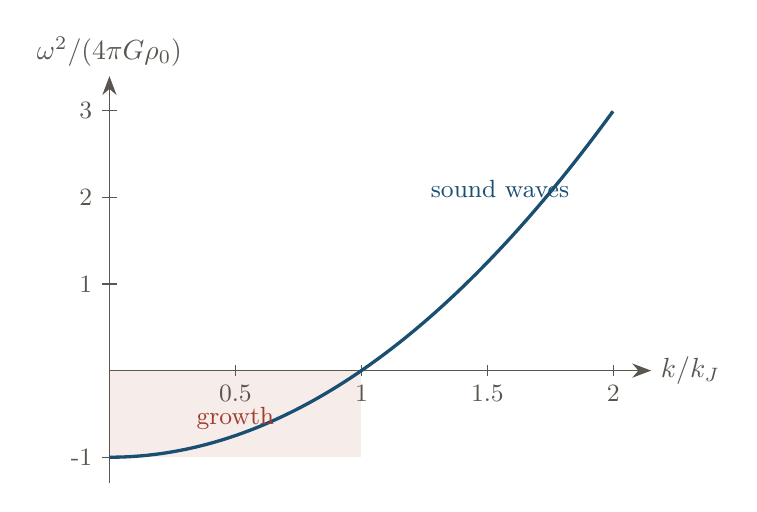
\begin{tikzpicture}[x=3.2cm,y=1.1cm, >={Stealth[length=2.4mm]}]
  \fill[accent!10] (0,-1) rectangle (1,0);
  \draw[->, muted] (0,0) -- (2.15,0) node[right] {$k/k_J$};
  \draw[->, muted] (0,-1.3) -- (0,3.4) node[above] {$\omega^2/(4\pi G\rho_0)$};
  \foreach \x in {0.5,1,1.5,2} \draw[muted] (\x,0.06) -- (\x,-0.06) node[below] {\small \x};
  \foreach \y in {-1,1,2,3} \draw[muted] (0.03,\y) -- (-0.03,\y) node[left] {\small \y};
  \draw[astroblue, line width=1.2pt, domain=0:2, samples=100] plot (\x, {\x*\x-1});
  \node[accent, align=center] at (0.5,-0.55) {\small growth};
  \node[astroblue] at (1.55,2.1) {\small sound waves};
\end{tikzpicture}
\end{document}
